\documentclass[11pt]{article}

\usepackage{amsmath}
\usepackage{amssymb}
\usepackage[margin=0.68in]{geometry}
\usepackage{booktabs}
\usepackage{enumitem}
\usepackage{fancyhdr}
\usepackage{graphicx}
\usepackage[table]{xcolor}
\usepackage[hidelinks]{hyperref}
\usepackage{listings}
\usepackage{microtype}
\usepackage{tabularx}
\usepackage{tikz}
\usepackage{titlesec}
\usetikzlibrary{arrows.meta,positioning}
\graphicspath{{docs/lessons/assets/}{../assets/}}

\definecolor{AdkBlue}{gray}{0}
\definecolor{AdkRed}{gray}{0}
\definecolor{AdkGreen}{gray}{0.20}
\definecolor{CodeGray}{gray}{0.96}
\definecolor{Soft}{gray}{0.92}
\hypersetup
{
    pdftitle={ADK Lesson 010: Shift Register Display},
    pdfauthor={Kevin Shanahan},
    pdfsubject={RAII shift-register output and nonblocking seven-segment display},
    pdflang={en-US}
}
\pagestyle{fancy}
\fancyhf{}
\lhead{\textsc{ADK Lesson 010}}
\rhead{Shift Register Display}
\cfoot{\thepage}
\setlength{\headheight}{14pt}
\setlength{\parindent}{0pt}
\setlength{\parskip}{5pt}
\setlist{nosep,leftmargin=1.45em}
\titleformat{\section}{\Large\bfseries\color{AdkBlue}}{\thesection}{0.5em}{}
\titleformat{\subsection}{\large\bfseries\color{AdkBlue}}{\thesubsection}{0.5em}{}
\lstdefinestyle{adkcpp}
{
    language=C++,
    backgroundcolor=\color{CodeGray},
    basicstyle=\ttfamily\small,
    keywordstyle=\color{AdkBlue}\bfseries,
    commentstyle=\color{AdkGreen},
    columns=fullflexible,
    keepspaces=true,
    showstringspaces=false,
    frame=single,
    rulecolor=\color{black!20},
    breaklines=true,
    tabsize=4
}
\newcommand{\checkbox}{\(\square\)}
\newcommand{\blank}[1]{\rule{#1}{0.4pt}}
\newcommand{\warningbox}[1]{%
  \begin{center}
  \fcolorbox{AdkRed}{AdkRed!6}{\parbox{0.91\linewidth}{\textbf{\color{AdkRed}Safety checkpoint.} #1}}
  \end{center}}
\newcommand{\evidencebox}[1]{%
  \begin{center}
  \fcolorbox{AdkBlue}{AdkBlue!5}{\parbox{0.91\linewidth}{#1}}
  \end{center}}

\begin{document}

\begin{center}
  {\Huge\bfseries Shift Register Display}\\[4pt]
  {\Large Send one bit at a time; reveal one stable digit}\\[8pt]
  \textit{The displayed glyph and three named test points explain the transfer without Serial.}
\end{center}

\begin{tabularx}{\linewidth}{@{}>{\bfseries}l X >{\bfseries}l X@{}}
Lesson & 010 --- component & Time & 120--180 minutes\\
Prerequisites & Lessons 001--009 & Board & Arduino Mega 2560\\
Evidence & glyph, TP-DATA, TP-CLOCK, TP-LATCH & Status & host verified; bench open\\
Safety & E1: USB-powered logic and resistor-limited LED segments only\\
\end{tabularx}

\section{Mission and evidence chain}

Build a decimal counter from two high-level objects:
\texttt{ShiftRegisterOutput} owns the three control pins, while
\texttt{SevenSegmentDisplay} turns a glyph into the register's eight output
bits. The sketch reads in the same order as the circuit:
\[
\text{time}\rightarrow\text{choose digit}\rightarrow
\text{serialize bits}\rightarrow\text{latch once}\rightarrow\text{stable glyph}.
\]

The D13 diagnostic LED proves that both components acquired their pins. The
display proves the current glyph. TP-DATA, TP-CLOCK, and TP-LATCH expose the
electrical transfer to a logic probe or oscilloscope. These observations prove
different claims; none alone proves the entire chain.

\subsection{Learning outcomes}

You will be able to:
\begin{itemize}
  \item distinguish a shift clock from the output latch;
  \item predict the register byte for a decimal glyph;
  \item explain why the visible display remains stable while new bits shift;
  \item use deterministic RAII ownership and a nonblocking update loop;
  \item separate acquisition, behavior, and safe-state evidence.
\end{itemize}

\warningbox{Identify the exact 74HC595 and display part numbers before wiring.
Seven-segment package pinouts vary. A common-anode display wired as
common-cathode gives misleading results and can exceed an LED rating. Remove
USB power before moving wires or meter clips.}

\section{Parts and current budget}

\begin{tabularx}{\linewidth}{@{}l l X@{}}
\toprule
Quantity & Part & Requirement\\
\midrule
1 & Arduino Mega 2560 & USB-powered reference board\\
1 & 74HC595 & 5 V HC-family eight-bit serial-in/parallel-out register\\
1 & Seven-segment display & One digit, common cathode, known pinout\\
8 & 470 \(\Omega\) resistors & One per segment, including decimal point\\
1 & Breadboard and jumpers & Short, inspectable connections\\
1 & Logic probe or oscilloscope & Optional; multimeter still verifies static levels\\
\bottomrule
\end{tabularx}

For each lit segment, calculate
\[
I_{\mathrm{segment}}=\frac{V_{\mathrm{CC}}-V_F}{470\ \Omega}.
\]
Record the actual LED forward-voltage specification. The lesson limit is
8\,mA per segment and 40\,mA total display current; increase the resistor value
if either calculation exceeds its limit. These conservative lesson limits do
not replace the register and display datasheets.

\newpage
\section{Authoritative wiring}

\begin{center}
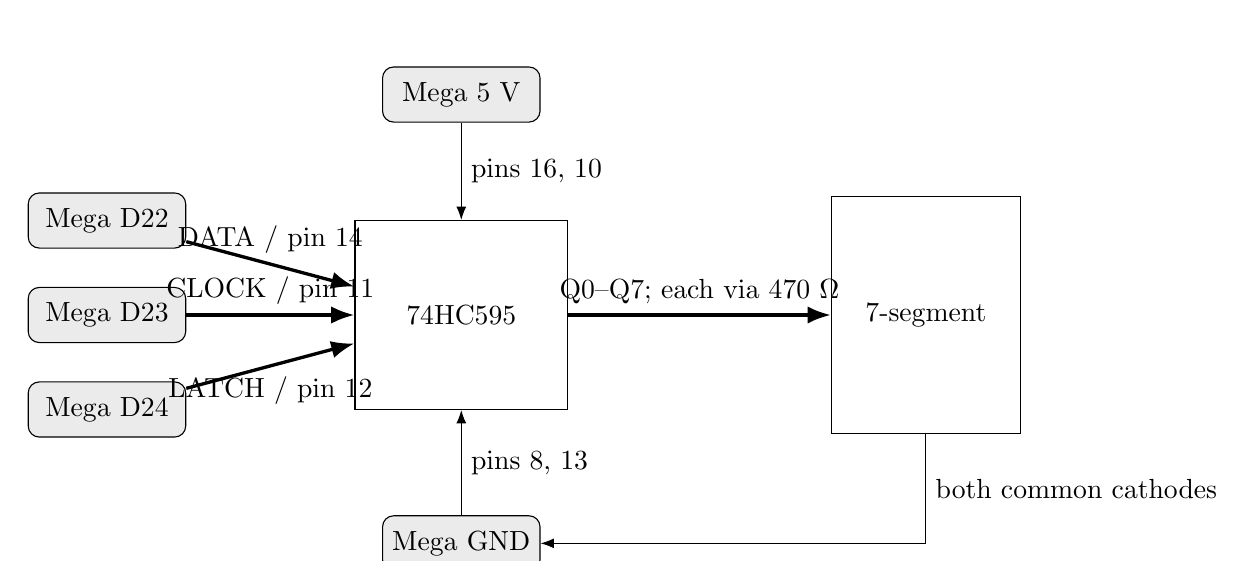
\begin{tikzpicture}[>=Latex,
    pin/.style={draw,rounded corners,fill=Soft,minimum width=20mm,minimum height=7mm},
    chip/.style={draw,fill=white,minimum width=27mm,minimum height=24mm},
    display/.style={draw,fill=white,minimum width=24mm,minimum height=30mm}]
  \node[pin] (d22) at (0,2.4) {Mega D22};
  \node[pin] (d23) at (0,1.2) {Mega D23};
  \node[pin] (d24) at (0,0.0) {Mega D24};
  \node[chip] (sr) at (4.5,1.2) {74HC595};
  \node[display] (seg) at (10.4,1.2) {7-segment};
  \draw[->,very thick] (d22)--node[above]{DATA / pin 14}(sr);
  \draw[->,very thick] (d23)--node[above]{CLOCK / pin 11}(sr);
  \draw[->,very thick] (d24)--node[below]{LATCH / pin 12}(sr);
  \draw[->,very thick] (sr)--node[above]{Q0--Q7; each via 470 \(\Omega\)}(seg);
  \node[pin] (vcc) at (4.5,4.0) {Mega 5 V};
  \node[pin] (gnd) at (4.5,-1.7) {Mega GND};
  \draw[->] (vcc)--node[right]{pins 16, 10}(sr);
  \draw[->] (gnd)--node[right]{pins 8, 13}(sr);
  \draw[->] (seg)--node[right]{both common cathodes}(10.4,-1.7)--(gnd);
\end{tikzpicture}
\end{center}

\textbf{Pin-by-pin connection list}
\begin{itemize}
  \item D22 / TP-DATA \(\rightarrow\) DS, 74HC595 pin 14.
  \item D23 / TP-CLOCK \(\rightarrow\) SHCP, pin 11.
  \item D24 / TP-LATCH \(\rightarrow\) STCP, pin 12.
  \item 5 V \(\rightarrow\) VCC pin 16 and active-low clear pin 10.
  \item GND \(\rightarrow\) GND pin 8 and active-low output-enable pin 13.
  \item Q0 through Q6 \(\rightarrow\) segments a through g; Q7
        \(\rightarrow\) decimal point. Every path has its own 470 \(\Omega\)
        resistor.
  \item Both display common-cathode pins \(\rightarrow\) GND. Use the display
        datasheet to locate them.
\end{itemize}

Place a 100\,nF ceramic bypass capacitor directly between pins 16 and 8. The
pencil plate helps with physical orientation only. In this introductory
three-wire circuit, active-low OE is tied to GND, so the output drivers are
enabled before the sketch runs. The 74HC595 storage register's power-up state
is not specified; reset or power-up can therefore show an arbitrary, possibly
bright, segment pattern until the first blank or glyph is latched. The
software lifecycle cannot prevent that startup transient.

A later hardware upgrade gives OE its own Mega output and a pull-up resistor.
The pull-up keeps the register outputs disabled while the Mega resets; software
then shifts and latches the blank value before driving OE low. That fourth
control signal is required when blank output during power-up is part of the
circuit contract.

\begin{center}
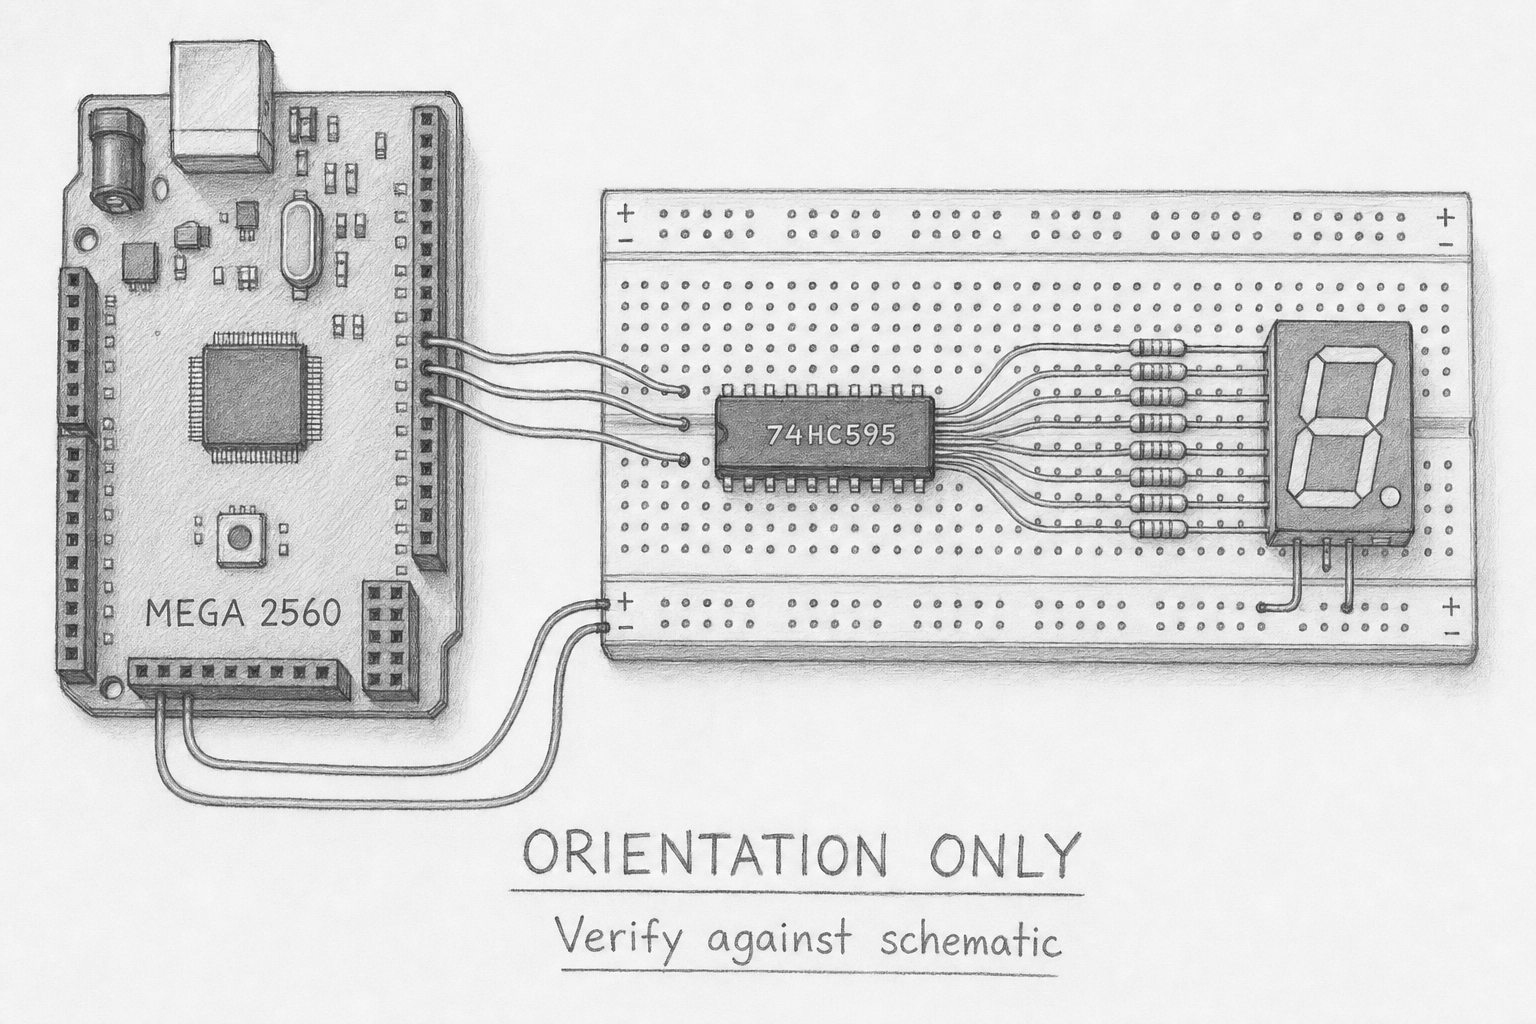
\includegraphics[width=0.89\linewidth]{010-shift-register-pencil.png}

\small\textit{Alternative text: a Mega, breadboard, 74HC595, eight resistors,
and one-digit display arranged left to right; the exact list above is authoritative.}
\end{center}

\newpage
\section{Interface and ownership}

\begin{lstlisting}[style=adkcpp]
constexpr adk::ShiftRegisterPins displayPins = {22, 23, 24};

adk::Runtime             runtime;
adk::SevenSegmentDisplay display (
    runtime.resources (),
    displayPins,
    adk::SevenSegmentPolarity::CommonCathode);

display.initialize ();
display.show (adk::SevenSegmentGlyph::Five);
display.blank ();
display.shutdown ();
\end{lstlisting}

\texttt{SevenSegmentDisplay} composes one \texttt{ShiftRegisterOutput}.
Initialization claims D22, D23, and D24 transactionally. A conflict leaves no
partial claim. Repeated initialization succeeds without another transfer.
\texttt{show()} accepts digits, hexadecimal glyphs, dash, blank, and an optional
decimal point.

For common cathode, a one bit lights its segment. For common anode the API
inverts all eight output bits. The wiring and constructor polarity must agree.
The supported mapping is Q0--Q6 to a--g and Q7 to the decimal point.

\texttt{shutdown()} first shifts the polarity-correct blank value, then makes
DATA, CLOCK, and LATCH high impedance and releases their claims. Destruction
does the same during normal scope exit or exception unwinding in a caller.
ADK itself neither throws nor allocates.

\subsection{A transfer without update flicker}

For each byte, \texttt{ShiftRegisterOutput::show()} holds LATCH low, presents
the most-significant remaining bit on DATA, and pulses CLOCK. After eight
clock pulses it pulses LATCH once. The output register changes as one visible
step, so intermediate shifted bytes are not shown during normal updates. This
does not control the register's unspecified state before the first software
latch while OE remains tied low.

\evidencebox{\textbf{Predict:} glyph 8 uses segments a--g, so its common-cathode
value is \texttt{0x7f}. \textbf{Observe:} seven segments lit and decimal point
dark. \textbf{Interpret:} the stable output matches the glyph encoding. It does
not prove clock timing margins; TP-CLOCK and TP-LATCH supply that evidence.}

\section{Narrative run loop}

The canonical sketch declares the runtime, display, and diagnostic LED in
dependency order. \texttt{setup()} reads ``acquire circuit, show ready.''
\texttt{loop()} reads ``observe time, decide whether the count is due, choose
the digit, show the digit.'' No \texttt{delay()} blocks observation.

\begin{lstlisting}[style=adkcpp]
void loop ()
{
    if (!ready)
    {
        return;
    }

    const adk::TimePoint now (millis ());

    if (!countIsDue (now))
    {
        return;
    }

    const adk::SevenSegmentGlyph digit = chooseDigit ();
    showDigit (digit);
}
\end{lstlisting}

The complete, compile-authoritative sketch is
\href{https://spincyc.github.io/adk/downloads/examples/Lesson010ShiftRegisterDisplay.ino}
{the Lesson 010 sketch download}. Build and upload it only through repository
targets; no particular IDE is required.

\newpage
\section{CLI experiment}

\begin{lstlisting}[style=adkcpp,language=bash]
make bootstrap
make arduino-Lesson010ShiftRegisterDisplay
make upload-Lesson010ShiftRegisterDisplay PORT=/dev/ttyACM0
make observe-new LESSON=010
make observe-check CARD=hardware/acceptance/lesson-010.md
\end{lstlisting}

Serial is optional supporting evidence:
\begin{lstlisting}[style=adkcpp,language=bash]
make monitor PORT=/dev/ttyACM0 BAUD=115200
make serial-log PORT=/dev/ttyACM0 BAUD=115200
\end{lstlisting}
The canonical sketch does not require or emit Serial messages. A missing serial
log therefore says nothing about display correctness.

\subsection{Predict, observe, interpret}

\begin{tabularx}{\linewidth}{@{}p{0.16\linewidth} X X@{}}
\toprule
Place & Prediction & Interpretation\\
\midrule
D13 & Steady on after setup & All four output pins were acquired; not proof of segment wiring\\
Display & 0, then one increment each second & Glyph selection and latched outputs agree visibly\\
TP-DATA & Eight data levels per update & Serialized value is present; probe with GND reference\\
TP-CLOCK & Exactly eight pulses per update & Eight bits were shifted\\
TP-LATCH & One pulse after the eight clocks & The visible output changes atomically\\
D22--D24 after shutdown & High impedance & Endpoint safe state; measure rather than infer from blank display\\
\bottomrule
\end{tabularx}

\subsection{Experiment sequence}

\begin{enumerate}
  \item With USB removed, inspect every IC pin, resistor, display common, and
        the bypass capacitor against the exact part datasheets.
  \item Predict the first three glyphs and the CLOCK:LATCH pulse count.
  \item Attach probes with power removed. Reference every measurement to Mega
        GND. Apply USB power only after a second inspection.
  \item Confirm D13 first, then the visible 0--9 sequence.
  \item Observe TP-DATA, TP-CLOCK, and TP-LATCH. Save one annotated capture.
  \item Remove USB power. Do not move bare probes around the live breadboard.
\end{enumerate}

\textbf{Host-verified is the current release status.} Do not fill the measured
columns or mark hardware accepted until the actual Mega circuit has been
observed and recorded.

\newpage
\section{Diagnosis by evidence}

\begin{tabularx}{\linewidth}{@{}p{0.23\linewidth} p{0.27\linewidth} X@{}}
\toprule
Observation & Distinguishes & Next check\\
\midrule
D13 dark & acquisition failed or setup stopped & pin conflicts, exact status in host test, then D13 circuit\\
D13 on; display dark & control acquired but display path unknown & 5 V/GND, OE low, clear high, display polarity\\
Wrong stable glyph & output path exists; mapping differs & Q0--Q7 order and segment a--dp datasheet pins\\
Partial glyph & one or more segment paths absent & resistor, LED segment, Q output continuity unpowered\\
Flicker or mixed glyph & latch behavior or supply integrity suspect & TP-LATCH pulse count and 100 nF bypass\\
No CLOCK pulses & transfer did not occur & TP-DATA/TP-CLOCK, initialization, pin conflict\\
Eight clocks; no latch & shift register changed internally only & TP-LATCH wiring and pin 12\\
Chip or resistor hot & unsafe current or wiring & remove USB immediately; recheck identity and current budget\\
\bottomrule
\end{tabularx}

\subsection{Fault injections without rewiring live}

\begin{itemize}
  \item In a host test, pre-claim CLOCK. Expect \texttt{ResourceBusy}, no
        partial DATA/LATCH ownership, and no output transfer.
  \item Construct an object with duplicate data and clock pins. Expect
        \texttt{InvalidArgument} before a claim or hardware write.
  \item Request every glyph twice and compare the recording fake's traces.
        They must match byte for byte.
  \item Advance timestamps across 32-bit wrap in the example timing model.
        The elapsed-time decision must remain correct.
\end{itemize}

\section{Design exercises}

\begin{enumerate}
  \item Write the common-cathode bytes for 0, 1, 2, and dash. Then invert each
        byte for common anode.
  \item Why is one resistor on the display common pin not equivalent to one
        resistor per segment?
  \item Extend the counter to hexadecimal without changing
        \texttt{ShiftRegisterOutput}.
  \item Add a decimal-point heartbeat that does not block the counter. Name
        the independent state and deadline.
  \item Sketch two cascaded 74HC595 registers. Which signal is shared, which
        output feeds the next DATA input, and which resource remains owned?
  \item Explain what a stable digit proves that a TP-CLOCK capture does not,
        and vice versa.
\end{enumerate}

\newpage
\section{Bench acceptance record}

\begin{tabularx}{\linewidth}{@{}l X l X@{}}
Date & \blank{1.25in} & Reviewer & \blank{1.35in}\\[7pt]
Board & Mega 2560 revision: \blank{1.0in} & USB supply & \blank{1.05in}\\[7pt]
74HC595 marking & \blank{1.4in} & Display marking & \blank{1.15in}\\[7pt]
Display polarity & \blank{1.2in} & Resistors & \blank{1.15in}\\[7pt]
Measured 5 V & \blank{1.2in} & Segment \(V_F\) & \blank{1.15in}\\[7pt]
Segment current & \blank{1.05in} & Maximum total & \blank{1.15in}\\
\end{tabularx}

\subsection{Required observations}

\begin{tabularx}{\linewidth}{@{}p{0.44\linewidth} c X@{}}
\toprule
Check & Pass & Recorded evidence\\
\midrule
Unpowered wiring matches both datasheets & \checkbox & \\
D13 separately proves successful acquisition & \checkbox & \\
Digits 0--9 are stable and correctly mapped & \checkbox & \\
TP-CLOCK shows eight pulses per update & \checkbox & \\
TP-LATCH shows one later pulse per update & \checkbox & \\
Startup transient with OE tied low is observed and recorded & \checkbox & \\
First software latch establishes the documented zero & \checkbox & \\
Reset returns to the documented initial sequence & \checkbox & \\
Shutdown blanks, then D22--D24 become high impedance & \checkbox & \\
Power removal leaves every part cool and dark & \checkbox & \\
\bottomrule
\end{tabularx}

\textbf{Instrument and capture identifiers:}
\blank{4.2in}

\textbf{Deviations or open questions:}
\vspace{0.55in}

\textbf{Stop conditions:} unexpected heat, unstable USB, a display current
above the recorded budget, signal outside the rails, unexpected simultaneous
segments, or disagreement between the actual part datasheet and this lesson.
Remove USB power physically; software shutdown is not the emergency stop.

\textbf{Deferred upgrade:} repeat the startup and reset observations after
adding a pulled-up, software-owned OE signal. Record that outputs remain
disabled until a blank byte has been shifted and latched; do not transfer that
claim to the three-wire circuit above.

\section{What comes next}

Lesson 011 keeps this display visible while a deterministic, nonblocking
traffic state advances and records pedestrian requests. Lesson 012 composes
the display, buttons, and mutually exclusive signal lamps into the next
three-lesson project.

\end{document}
